\chapter{Experiments}\label{chap:experiments}
A series of experiments were carried out to determine the performance of the network in its stated goal of classifying curbs and curb cuts. To this end, the network was tested on the Mapillary Vistas dataset \cite{mapillary} and its hyperparameters optimized using the Bayesian optimization with hyperband (BOHB) procedure from the AutoML group at the University of Freiburg \cite{bohb}

\section{Dataset} \label{section:experiments-dataset}
The Mapillary Vistas dataset was chosen for this task as it was, to our knowledge, the only street-level dataset that included ground truth segmentations of both curbs and curb cuts.
This dataset contains images from all around the world and includes images captured from different imaging devices including mobile phones, action cameras, and professional imaging solutions.
These images are captured during various weather, seasonal, and daylight conditions.
As such, the dataset provides a challenging level of diversity.

With such a diverse dataset, the images must first be preprocessed.
We process all the images to conform to a 4:3 size ratio, eliminate images without images of curbs or curb cuts, and extract only road, curb, and curb cut classes.

To optimize training speed with respect to wall clock time, and given the computational constraints, images were resized for training.
The chosen image resolution was $360 \times 320$ pixels. 
This allows a batch size of 16 per GPU, given that the GPU has 12 GB of VRAM.
To further optimize training, the images are resized prior to training and the resized images stored.
This allows all training and validation images to be loaded into memory, reducing the number of file accesses required and reducing training wall clock time by a factor of two.

After running an analysis of the dataset with respect to their curb and curb cut content and image dimensions, we found that there were 15,160 usable images in the training set and 1610 usable images in the validation set.
Usable images in this case refers to images that contains both curbs and curb cuts.
A detailed results of the analysis of can be found in Appendix section \ref{appendix:dataset}.

\section{Network Evaluation}\label{section:experiments-networkevaluation}
Experiments were done to evaluate the performance of different networks on our dataset.
Specifically, we identified the small size of curbs relative to the rest of the image causes a severe class imbalance and increases the difficulty in recognizing the smaller features.

Relative to the entire image, curb and curb cut classes make up a relatively small proportion of the image, making up 0.986\% and 0.196\% of images on average respectively.
As such, three networks with good known performance for urban scene segmentation were chosen and evaluated for their performance classifying curbs and curb cuts.
We experimented with GoogLeNet, described in the paper "Going Deeper with Convolutions"~\cite{googlenet}; FCN16s, described in "Fully Convolutional Networks for Semantic Segmentation"~\cite{fcn}; and DeepLab v3+, described in the paper "Encoder-Decoder with Atrous Separable Convolution for Semantic Image Segmentation"~\cite{deeplab}.

To evaluate which network would have the most potential, we trained each network on a small subset of the whole dataset to find which networks would converge the fastest given a certain budget.
For each of these runs, the default recommended hyperparameters were used due to time constraints to conduct hyper-parameter optimization with every network.
The results can be seen in \figref{chart:experiments-networkcomparison} and in \tabref{tab:network-comparison}.
Given these results, we chose to use DeepLab v3+ as our network.

% Please add the following required packages to your document preamble:
% \usepackage{booktabs}
% \usepackage{graphicx}
\begin{table}[b]
	\centering
	\begin{tabular}{@{}ll@{}}
		\toprule
		Network     & mIoU \\ \midrule
		DeepLab v3+ & 30.83\%   \\
		FCN16s      & 19.97\%   \\
		GoogLeNet   & 25.08\%   \\ \bottomrule
	\end{tabular}
	\caption[Network Comparison Results]{Results of running the DeepLab v3+, FCN16s, and GoogLeNet on a subset of the main dataset after one thousand iterations. It can be seen that DeepLab v3+ was able to achieve the highest mIoU performance overall.}
	\label{tab:network-comparison}
\end{table}
\begin{figure}
	\centering
	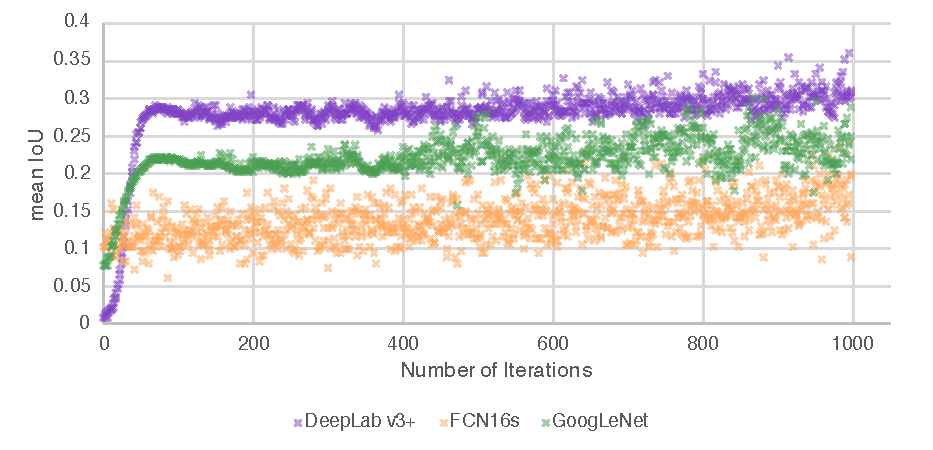
\includegraphics[width=\textwidth]{figures/experiments/network-comparison.pdf}
		\caption[Network Comparison Chart]{Training mIoU Accuracy over 1000 Iterations using DeepLab v3+, FCN16s, and GoogLeNet. It can be seen that DeepLab v3+ achieves the best mIoU performance overall.}
		\label{chart:experiments-networkcomparison}
\end{figure}

\section{Modifications to DeepLab v3+}\label{section:experiments-modifications}
Given that we are working with the assumption of a camera with a constant attitude, we can also make the assumption that curbs will be more likely towards the bottom and sides of an image.
Therefore, modifications were made to DeepLab v3+ by adding a preprocessing step which turns the input image into a five-dimensional tensor, with the fourth and fifth dimensions being the $x$ and $y$ coordinates of the pixel, respectively.
The initial convolutional layer was also modified to accept five channels as input.
Both versions of the network were run with identical hyperparameters on a limited budget and dataset.
While there was an increase in mean IoU accuracy when using the five-dimensional input tensor, it was negligible and we decided to use the three-dimensional input tensor, given the increased training time with a five-dimensional input tensor.

\todo{include 5D vs 3D results}

\section{Loss Function Evaluation}\label{section:experiments-loss}
Our custom loss function masked cross entropy loss was evaluated against weighted cross entropy loss.
The results, shown in \figref{chart:experiments-losstraining} and \ref{chart:experiments-lossvalidation}.
These results show that the validation loss was similar for the first 2370 iterations.
After this point, masked cross entropy loss shows a clear advantage in validation accuracy compared to weighted cross entropy loss.
After 4740 iterations, shows a clear performance advantage, with a difference of 5.56 mean IoU percentage points.
As such, we have chosen to implement our network using masked cross entropy loss as our loss function.

\begin{figure}
	\centering
	\begin{subfigure}{\textwidth}
		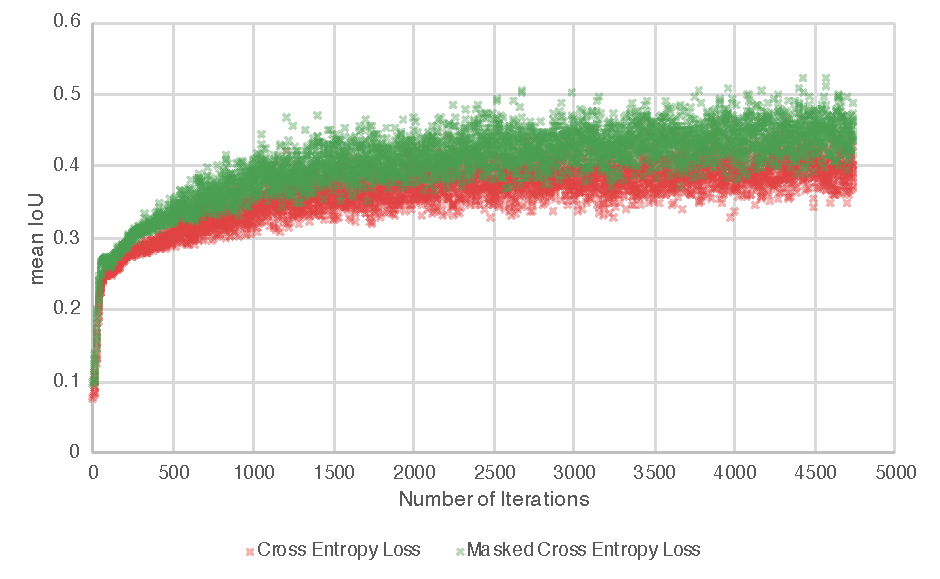
\includegraphics[width=\textwidth]{figures/experiments/loss-comparison-training.pdf}
		\caption[Loss Comparison Chart: Training]{Training mIoU Accuracy over 4740 Iterations comparing weighted cross entropy loss and masked cross entropy loss. The results show that although performing similarly to begin with, masked cross entropy loss was able to outperform weighted cross entropy loss.}
		\label{chart:experiments-losstraining}
	\end{subfigure}
	\newline
	\begin{subfigure}{\textwidth}
		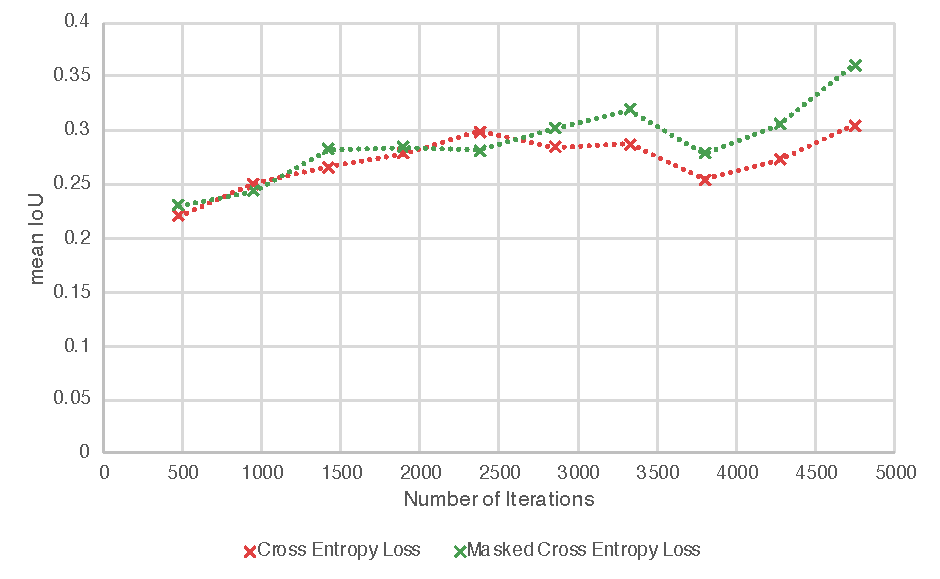
\includegraphics[width=\textwidth]{figures/experiments/loss-comparison-validation.pdf}
		\caption[Loss Comparison Chart: Validation]{Validation mean IoU Accuracy over 4740 Iterations, measured every 474 iterations, comparing cross entropy loss and masked cross entropy loss. Validation accuracy was evaluated against a validation set of 1680 images. The lines shown in the chart are to emphasize the data.}
		\label{chart:experiments-lossvalidation}
	\end{subfigure}
	\caption[Loss Comparison Chart]{Comparisons of masked cross entropy loss and weighted cross entropy loss. Both loss functions were evaluated using the same hyperparameters against a dataset consisting of 15160 training images and 1680 validation images.}
\end{figure}

\section{Hyperparameters} \label{section:experiments-hyperparameters}
Hyperparameter tuning was done by using Bayesian Optimization with HyperBand.
The hyperparameters that were tuned were the learning rate; optimizer; momentum, if the optimizer chosen was stochastic gradient descent; epsilon, if the optimizer chosen was Adam; the weight ratio for the loss weights; and the loss criterion.

The learning rate is optimized between the interval $\left[1 \times 10^{-5}, 1 \times 10^{-2}\right]$, varied on a logarithmic scale.
The optimizer is a categorical choice between stochastic gradient descent or Adam.
The momentum is optimized between the interval $\left[0, 0.99\right]$.
The epsilon value is optimized between the interval $\left[1 \times 10^{-2}, 1\right]$.
The weight ratio for the loss weight determines the ratio of the weights between the curb and curb cut.
The value of the weight for the "other" class is one-tenth of the sum of curb and curb cut weights, formally defined as:
\begin{equation}
	\begin{split}
		\frac{x}{y} &= r, ~r \in \left[2, 6\right]\\
		z &= \frac{x + y}{10}
	\end{split}
\end{equation}
where $x$ is the weight for the curb class, $y$ the weight for the curb cut class, $z$ the weight for the "other" class, and $r$ the ratio value that is optimized.
The loss criterion is a categorical choice between weighted cross entropy loss or masked cross entropy loss.
Further details of the hyperparameters optimized can be found in \tabref{tab:hyperparameters}.
\todo{make sure cross entropy loss or masked cross entropy loss}
% Please add the following required packages to your document preamble:
% \usepackage{booktabs}
\begin{table}[]
\begin{tabular}{@{}llp{3.9cm}p{3cm}@{}}
\toprule
Parameter Name    & Parameter Type & Range                                            & Comments                               \\ \midrule
Learning rate     & Float          & $\left[1 \times 10^{-5}, 1 \times 10^{-2}\right]$& On a logarithmic scale                \\
Optimizer         & Categorical    & Adam or SGD                                      &                                      \\
SGD momentum      & Float          & $\left[0, 0.99\right]$                           & Only active when the optimizer is SGD\\
Adam epsilon      & Float          & $\left[1 \times 10^{-2}, 1\right]$               & Only active when the optimizer is Adam\\
Loss weight ratio & Float          & $\left[2,6\right]$                               &                                       \\
Loss criterion    & Categorical    & Weighted cross entropy or masked cross entropy   &                                      \\ \bottomrule
\end{tabular}
\caption[Hyperparameter Details]{Table of hyperparameters and their values that were optimized for using Bayesian Optimization and HyperBand.}
\label{tab:hyperparameters}
\end{table}

\extend{include graph}
The hyperparameters are optimized according to the above parameters using a cluster of \todo{number of} GPUs over a budget of 12 iterations.
The resulting optimized values for the hyperparameters are in \tabref{tab:hyperparameterresults}.
More detailed results of each run of the hyperparameter optimization can be found in Appendix section \ref{appendix:hpoptimresults}.

Given increased compute resources and time, we believe that we could further optimize the hyperparameters and achieve better results with our network.

% Please add the following required packages to your document preamble:
% \usepackage{booktabs}
\begin{table}[]
	\centering
\begin{tabular}{@{}lp{2.3cm}}
\toprule
Parameter Name    & Value     \\ \midrule
Learning rate     & 0.0002    \\
Optimizer         & Adam      \\
SGD momentum      & -         \\
Adam epsilon      & 0.1       \\
Loss weight ratio & 4         \\
Loss criterion    & Masked cross entropy loss\\ \bottomrule
\end{tabular}
\caption[Hyperparameter Optimization Results]{Table of hyperparameters and their values that were optimized for using Bayesian Optimization and HyperBand. \todo{complete table values}}
\label{tab:hyperparameterresults}
\end{table}

\section{Training Pipeline} \label{section:experiments-trainingpipeline}
The training pipeline is a main script which calls the training loop with a set of parameters defined in either a JSON file or through command-line arguments.
Using a JSON file makes it simpler to change parameters as nothing is hard-coded and command-line arguments do not have to be memorized or meticulously typed out each time.

A Graphical User Interface (GUI) is also available, made using the tkinter framework, which is capable of visualizing the ground truth segmentation, the network output, a live display of the current loss and mean IoU accuracy, and other statistics.
This GUI can be seen in \figref{fig:experiments-gui}.

A Command Line Interface (CLI) is also available, made using the ncurses framework, which is capable of displaying various statistics during training.
The CLI also allows training remotely using secure shell (SSH), as the GUI would fail to start if invoked remotely through the command line.
A screen capture of the CLI can be seen in \figref{fig:experiments-cli}

\begin{figure}
	\centering
	\begin{subfigure}{0.45\textwidth}
		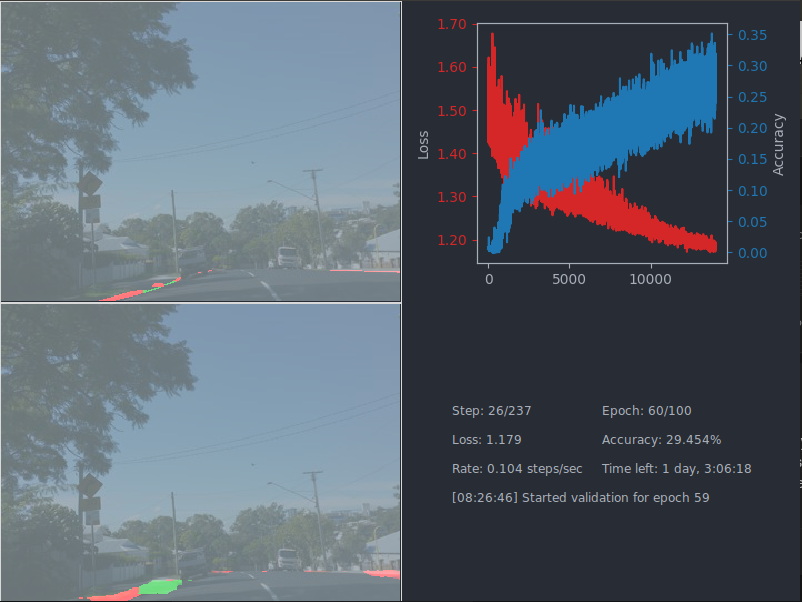
\includegraphics[width=\linewidth]{figures/experiments/gui.png}
		\caption[Training GUI]{A screen capture of the GUI that was used to visualize training results. In clockwise from the top left, the GUI visualizes the ground truth data, a live plot of the loss and accuracy, various statistics, and the network output.}
		\label{fig:experiments-gui}
	\end{subfigure}
	\hfill
	\begin{subfigure}{0.45\textwidth}
		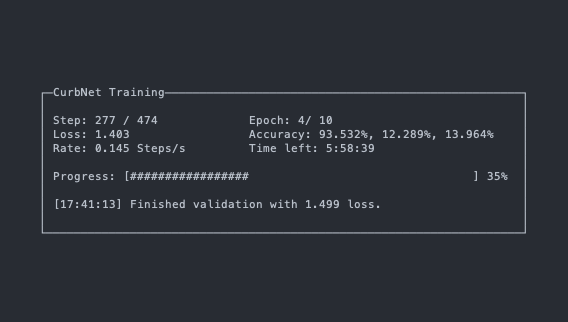
\includegraphics[width=\linewidth]{figures/experiments/cli.png}
		\caption[Training CLI]{A screen capture of the CLI that was used to train the network remotely.}
		\label{fig:experiments-cli}
	\end{subfigure}
	\caption[Training UI]{The two available user interfaces available to use with CurbNet. The GUI was mean to more simply and quickly deliver the most important information first to the researcher. The CLI was designed to allow training status along with the most pertinent information to be shown remotely with little overhead.}
\end{figure}

The different components necessary to train the network are written in such a way as to be modular, with nearly everything being easily configurable.
For example, the network, optimizer, and loss criterion can easily be swapped by changing command-line arguments or parameters in the JSON file.
This makes running different experiments straightforward.

\section{Evaluation Metrics} \label{section:experiments-evaluationmetrics}
The mean Intersection over Union (mIoU) is the main evaluation metric chosen.
IoU measures the intersection of the prediction and the ground truth data, divided by the union of the prediction and the ground truth data.
This is done on a per class basis and then averaged to get the mIoU.


\section{Results}\label{section:experiments-results}
Running our network with the optimal hyperparameters chosen by the hyperparameter search in Section \ref{section:experiments-hyperparameters} for \todo{how many iterations did we train} iterations, we were able to achieve an accuracy of \todo{value}.
We were able to train the network for \todo{how many before overfit} before the network started overfitting to the training set.

The network is able to produce the segmentations seen in \todo{include figure}.

Analyzing these results, we can see that the network excels at \todo{what does it excel at}.
Surprisingly, the network can even identify curbs and curb cuts which are in the distance and thus have a relatively small size.
In these cases, the segmentation is significantly larger than the size of the curb itself, i.e. even though the intersection is significant, there is a significant area around the curb that is falsely identified as part of the curb.
An example of this can be seen in \todo{figure}

The main failure modes of the network are falsely identifying non-curb road edges as curbs and identifying certain road markings as curbs.
Certain road edges which have a different texture, but are not raised, are sometimes also segmented as curbs.
Certain road markings which are located near road edges are also sometimes segmented as curbs.
Examples of both of these cases can be seen in figure \todo{figure}
We hypothesize that this may be a result of the network not having depth information.

Given depth information, it may be possible to reduce these false positives and further increase the performance of the network.
